\documentclass{article}
\usepackage{graphicx} % Required for inserting images
\usepackage{amsmath}
\usepackage{amssymb}
\title{Data Sampling? Statistics? Gambling!!??}
\author{Eric Yee}
\date{December 2023}
%\blrub{Sampling roulette tables? Sampling continuous random variables? Darts!}
\begin{document}

\maketitle

Sampling is a pretty intuitive concept. To explain it, I'll flashback to 10-year-old me, drunk and in a back alley casino.

I lean over the roulette wheel, clutching my head as I see my life savings taken away. \emph{How did it come to this?} I've rolled a 00 three out of the ten times I've rolled this wheel of my life, where there are a total of 37 notches. I'm unable to leave, desperately clinging on to ten years of my savings fitted into the chip rack. 

I try distracting myself with numbers. \emph{What the probability of rolling my three 00's?} Well there should be a $\frac{1}{37}$ chance of a $00$, and so $\frac{36}{37}$ chance of not rolling it. Multiplying by the permutations gave me an unlikely result of $\binom{10}{3}\left(\frac{1}{37}\right)^3\left(\frac{1}{37}\right)^7=0.002$. 

My mood worsened. I should never have emptied my entire piggy bank into chips. Am I doomed to waste my life at the ripe age of 10?

No! I will not simply take this as a lesson about gambling. My purpose is noble, and my heart is true. Luck cannot be so out of my favor. After half of the people leave, drudgingly, with empty pockets, followed by the other half which ripped their pockets from their tear-soaked hands, I slither my way back to the roulette table. With not even the managers left, I set my notebook on the rim of the wheel. Pulling out a synthetic ivory ball from my pocket, I spin the wheel 200 times, recording the results. 

I wrote down 5 times 00 was rolled, 97 times green was rolled, and 98 times red was rolled. Now I did some arithmetic expecting a rigged game and daydreaming about a very angry complaint to the Washington State Gambling Commission. $\frac{5}{200} = 0.025=\frac{1}{37}$, $\frac{97}{200} = 0.485=\frac{18}{37}$, $\frac{98}{200} = 0.49=\frac{18}{37}$.

\$@\$\#\%... I guess it wasn't rigged.

The point still stands though. Sampling takes the values of a random variable and generalizes to describe the random variable as a whole. Where in our case the random variable was the final notch our ball rolls on.

This might sound light right? WRONG! What if we want to sample a really disgusting random variable $X$ which has a probability density function of $f:(-2,2)\rightarrow \mathbb{R}_{>0}$:
$$f(x)=e^{-x^4}\left(\frac{1}{2}\cos^2(x) + 3\sin^2(x)\right)$$
\begin{center}
    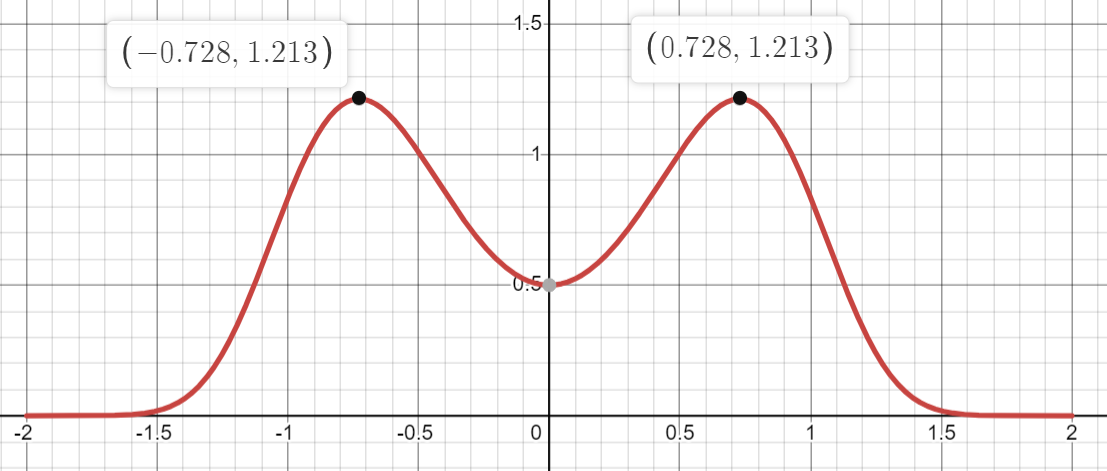
\includegraphics[width=10cm, scale=1.5]{images/ugly distribution.png}
\end{center}

Remember, when we sample, we want to compile a list of values of $X$ (which are the values on the x-axis) with a frequency that matches the density function.

Hmmm, this is difficult. To sample, as always, we'll have to go back to playing games. Consider creating a dart board behind this distribution, which has a length $4$, and a height $1.213$:
\begin{center}
    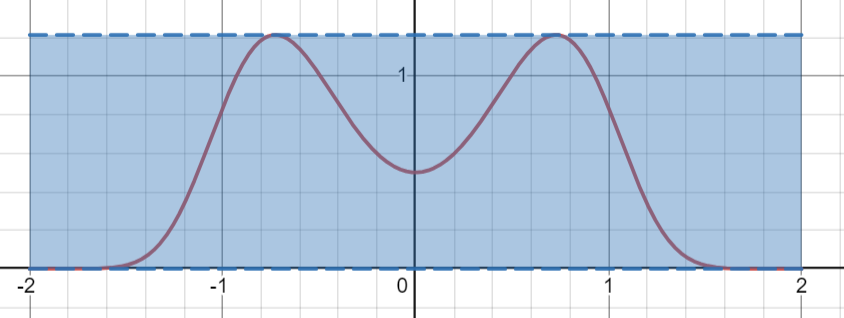
\includegraphics[width=10cm, scale=1.5]{images/ugly dartboard.png}
\end{center}

Now let's situate ourselves with a few hundred darts standing before the board. Due to how intoxicated we are, every throw lands at a uniformly random location on the rectangle. Like the monkeys we are, we begin throwing. Every time it lands above the distribution the dart bounces off and we try again. If it lands under the distribution the dart stays there. At the end we write down the x value of all the darts. Now notice that a part with a thicker distribution has a proportionally higher chance of being sampled than a thinner part, so thus we sampled the graph!

Ok, now you might be looking for some real-world examples since you've only heard one about a drunk ten-year-old hitting up the casino (which is pretty relatable). One that comes to mind is that people often prefer discreet models (ie. histograms) to continuous ones. To do this, we can sample the density function a lot of times and create a histogram at intervals of $X$ values with a height based on the number of times $X$ was sampled in that interval.

Enjoy the darts!... and statistics too!
\end{document}
